%!TEX root = ../thesis.tex

\section{テストフェーズ}
提案手法におけるテストフェーズでは\figref{Fig:suggest_test_phase}で示すように, 学習器の入力へ目標方向を加えた. なお, テストフェーズも学習フェーズと同様に, 地図を用いたルールベース制御器から目標方向を生成している. 本来ならば, 目的地までカメラ画像のみで自律移動するためには, 目標方向を画像から自動的に作成する仕組みが必要となる. 
% figに動作の様子を示す. 
カメラ画像と目標方向を入力した学習器の出力による自律走行時, 目標方向によって任意の経路を選択する.

\vspace{3cm}

\begin{figure}[hbtp]
  \centering
 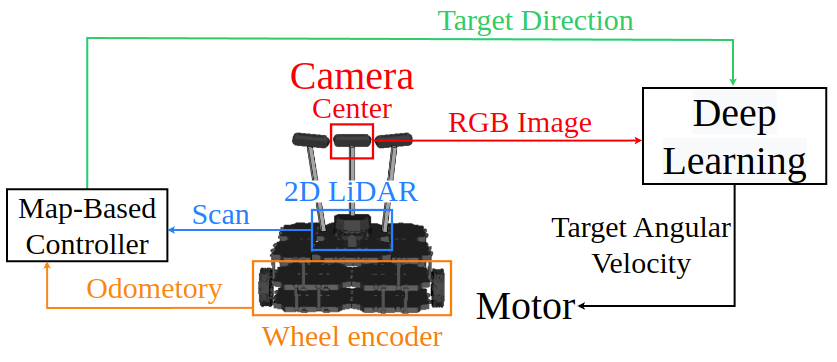
\includegraphics[keepaspectratio, scale=0.45]
      {images/suggest_test_phase.png}
 \caption{Learning phase system of proposed method}
 \label{Fig:suggest_test_phase}
\end{figure}

% \subsubsection{etc...}
\newpage
